\section{Electroviscous effect}
In section \ref{sec:et:streaming_pot}, the physical model behind
pressure-driven electrokinetic flow is presented. The effect of
interest that arise in this kind of systems is the electroviscous
effect.

Velocity profiles computed in a 1D situation is presented here. We
consider a 1 $\mu$m wide channel that has negatively charged
walls. The wall charge is a parameter that is varied and from this the
effect on the velocity profile is studied. The system is setup with a
Peclet number, $\Pe = 1$ and a Reynolds number, $\Rerm = 10^{-4}$. To
drive the flow, a pressure gradient of 1 kPa/m is set. The resulting
velocity profiles are presented in fig. \ref{fig:res:ev}.

\begin{figure}
\begin{center}
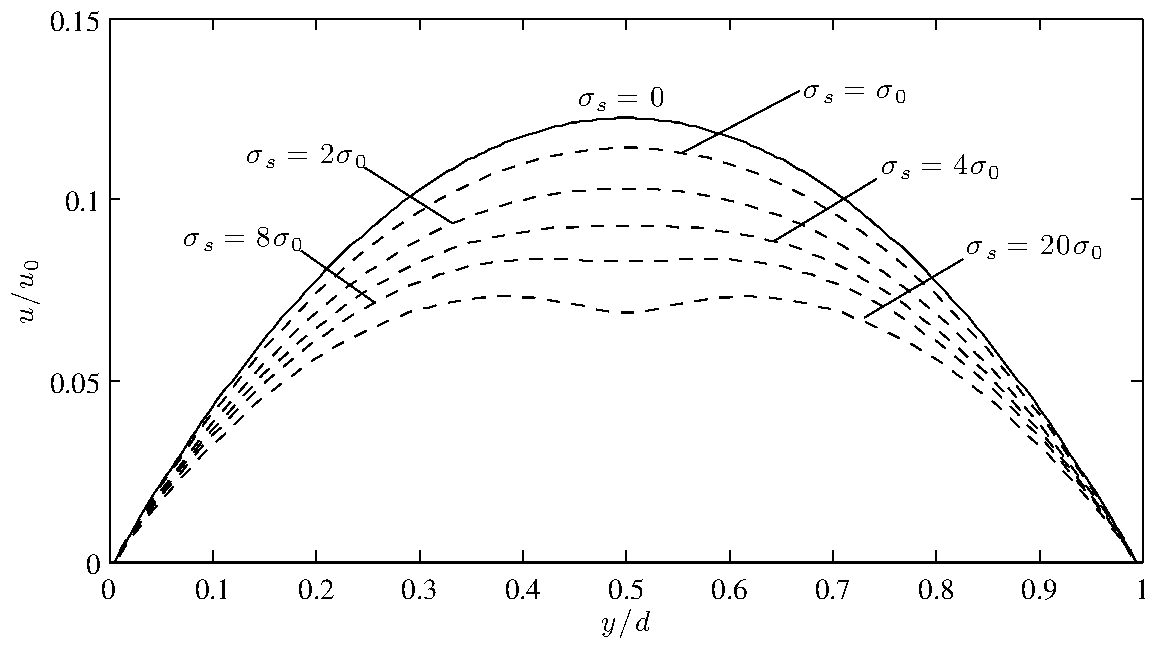
\includegraphics[width=0.9\textwidth]{fig/electrovisc.pdf}
\end{center}
\caption{Computed velocity profiles across a 2D channel of width $d =
  1 \mu$m. The flow is driven by a pressure gradient and the flow is
  slowed down due to the electroviscouos effect, this effects
  dependence on the surface charge $\sigma_s$ is here illustrated. The
  solution in the channel is a KCl solution defined by parameters in
  table \ref{tab:res:param}. In this simulation, $\sigma_0 = 0.89
  \mu$C/m$^2$, $\partial_xP = 1$ kPa/m and $u_0 = 10$ mm/s. }
\label{fig:res:ev}
\end{figure}

The velocity profiles obtained agrees qualitatively with a similar
simulation preformed in \cite{ren-elvis-paper}. The local minimum that
arises for $\sigma_s  = 20\sigma_0$ is due the high accumulation of
negative ions in the middle of the channel. This is an effect that
only is seen for narrow channels.

In the model proposed here, using Ohm's law to relate the ion current
to the streaming potential, the force on the flow due to the
electroviscous effect is opposite to the flow everywhere where there
is a net charge present in the fluid. However, in most texts about the
electroviscous effect, e.g. in \cite{dongquing-ren-book},
\cite{wang-poi} and \cite{ren-elvis-paper}, this force is computed
using a mean current approach. An integration of ion flux over the
cross-section of the channel is performed and then a net current for
the whole channel is obtained. From this current, a mean streaming
potential is obtained for the channel and a force is calculated using
the charge density. This gives that positive and negative net charged
regions of the fluid will be affected with forces of opposite sign
respectively. Having a mean streaming potential for the whole channel
also gives contraintuitve results when considering the fact that
regions in the fluid with the same net charge but different velocities
is affected by the same force. Also with this approach the
electroviscous effect would in principle be able to locally oppose the
flow direction. Also, in a more complicated geometry, this approach
would break down. In fig. \ref{fig:res:ev_comp}, two velocity profiles
from fig. \ref{fig:res:ev} are compared with corresponding profiles
computed using the mean current approach. It is seen that the
force slowing down flow is smaller for the case when using a mean
current. This is due to the cancellation between negative and
positive ion fluxes in the integration.

\begin{figure}
\begin{center}
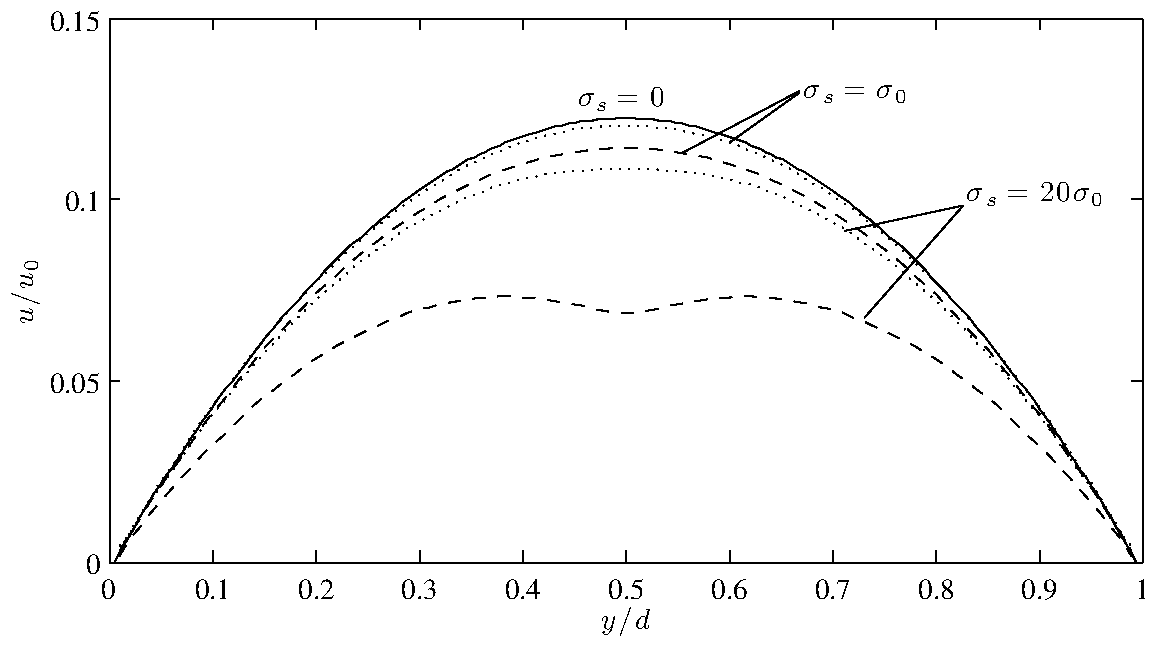
\includegraphics[width=0.9\textwidth]{fig/electrovisc_comp.pdf}
\end{center}
\caption{Comparison between velocity profiles computed using a mean
  current (dotted) and by using the actual local current (dashed) for
  the streaming potential. The solution in the channel is a KCl
  solution defined by parameters in table \ref{tab:res:param}. In this
  simulation, $\sigma_0 = 0.89 \mu$C/m$^2$, $\partial_xP = 1$ kPa/m
  and $u_0 = 10$ mm/s. }
\label{fig:res:ev_comp}
\end{figure}
